\section{问题二的建模与求解(交叉引用与图表排版简介)}

\subsection{交叉引用}

大家在前面的第~\ref{subsection1}~节已经初步见识到了交叉引用的作用,它以蓝色的编号作为标志,让阅读者点击编号可以直接跳转到指定位置,而这样的位置可以是“章”、“节”、“图”、“表”等。交叉引用主要有两种情况,下面我一一说明:

\subsubsection{图、表、章节的交叉引用}

这一类的交叉引用仅需在代码后面加上“杠label\{name\}”,这一点第~\ref{subsection1}~节中对数学公式的交叉引用我们已经介绍过,对于章节的交叉引用第~\ref{subsection1}~节也给了我们一个很好的示例。需要注意的是这个name必须是全文唯一!

进行label标注以后,我们可以在全文的任意地方进行引用,加上如上的代码就可以引用。

\subsubsection{参考文献的交叉引用}

这一类的交叉引用则是首先要在chapter文件夹中的第九个文件“9-参考文献.tex”中将参考文献按规范排版好,然后通过~\cite{ref1}~进行索引。






\subsection{插入图片}

我在模板文件中已经设置好图片文件的储存路径,也就是与“数学建模竞赛论文模板参考.tex”同处一个文件夹的Figures文件夹,要想在\LaTeX 插入图片,首先要把图片放在这个文件夹中!接下来要做的就是复制我下面写好的代码,并修改三个地方即可。

这里要注意,插入图的时候尽量使用矢量图,因为这样的图任意放大、缩小都不会模糊。特别是基于Python实现数据可视化时,尽量导出eps格式的矢量图,如图~\ref{fig2}~所示:

\begin{figure}[H] 
	\centering 
	% 这个1.eps修改为你要插入在这个位置的图片的文件名,该文件必须在Figures文件夹中
	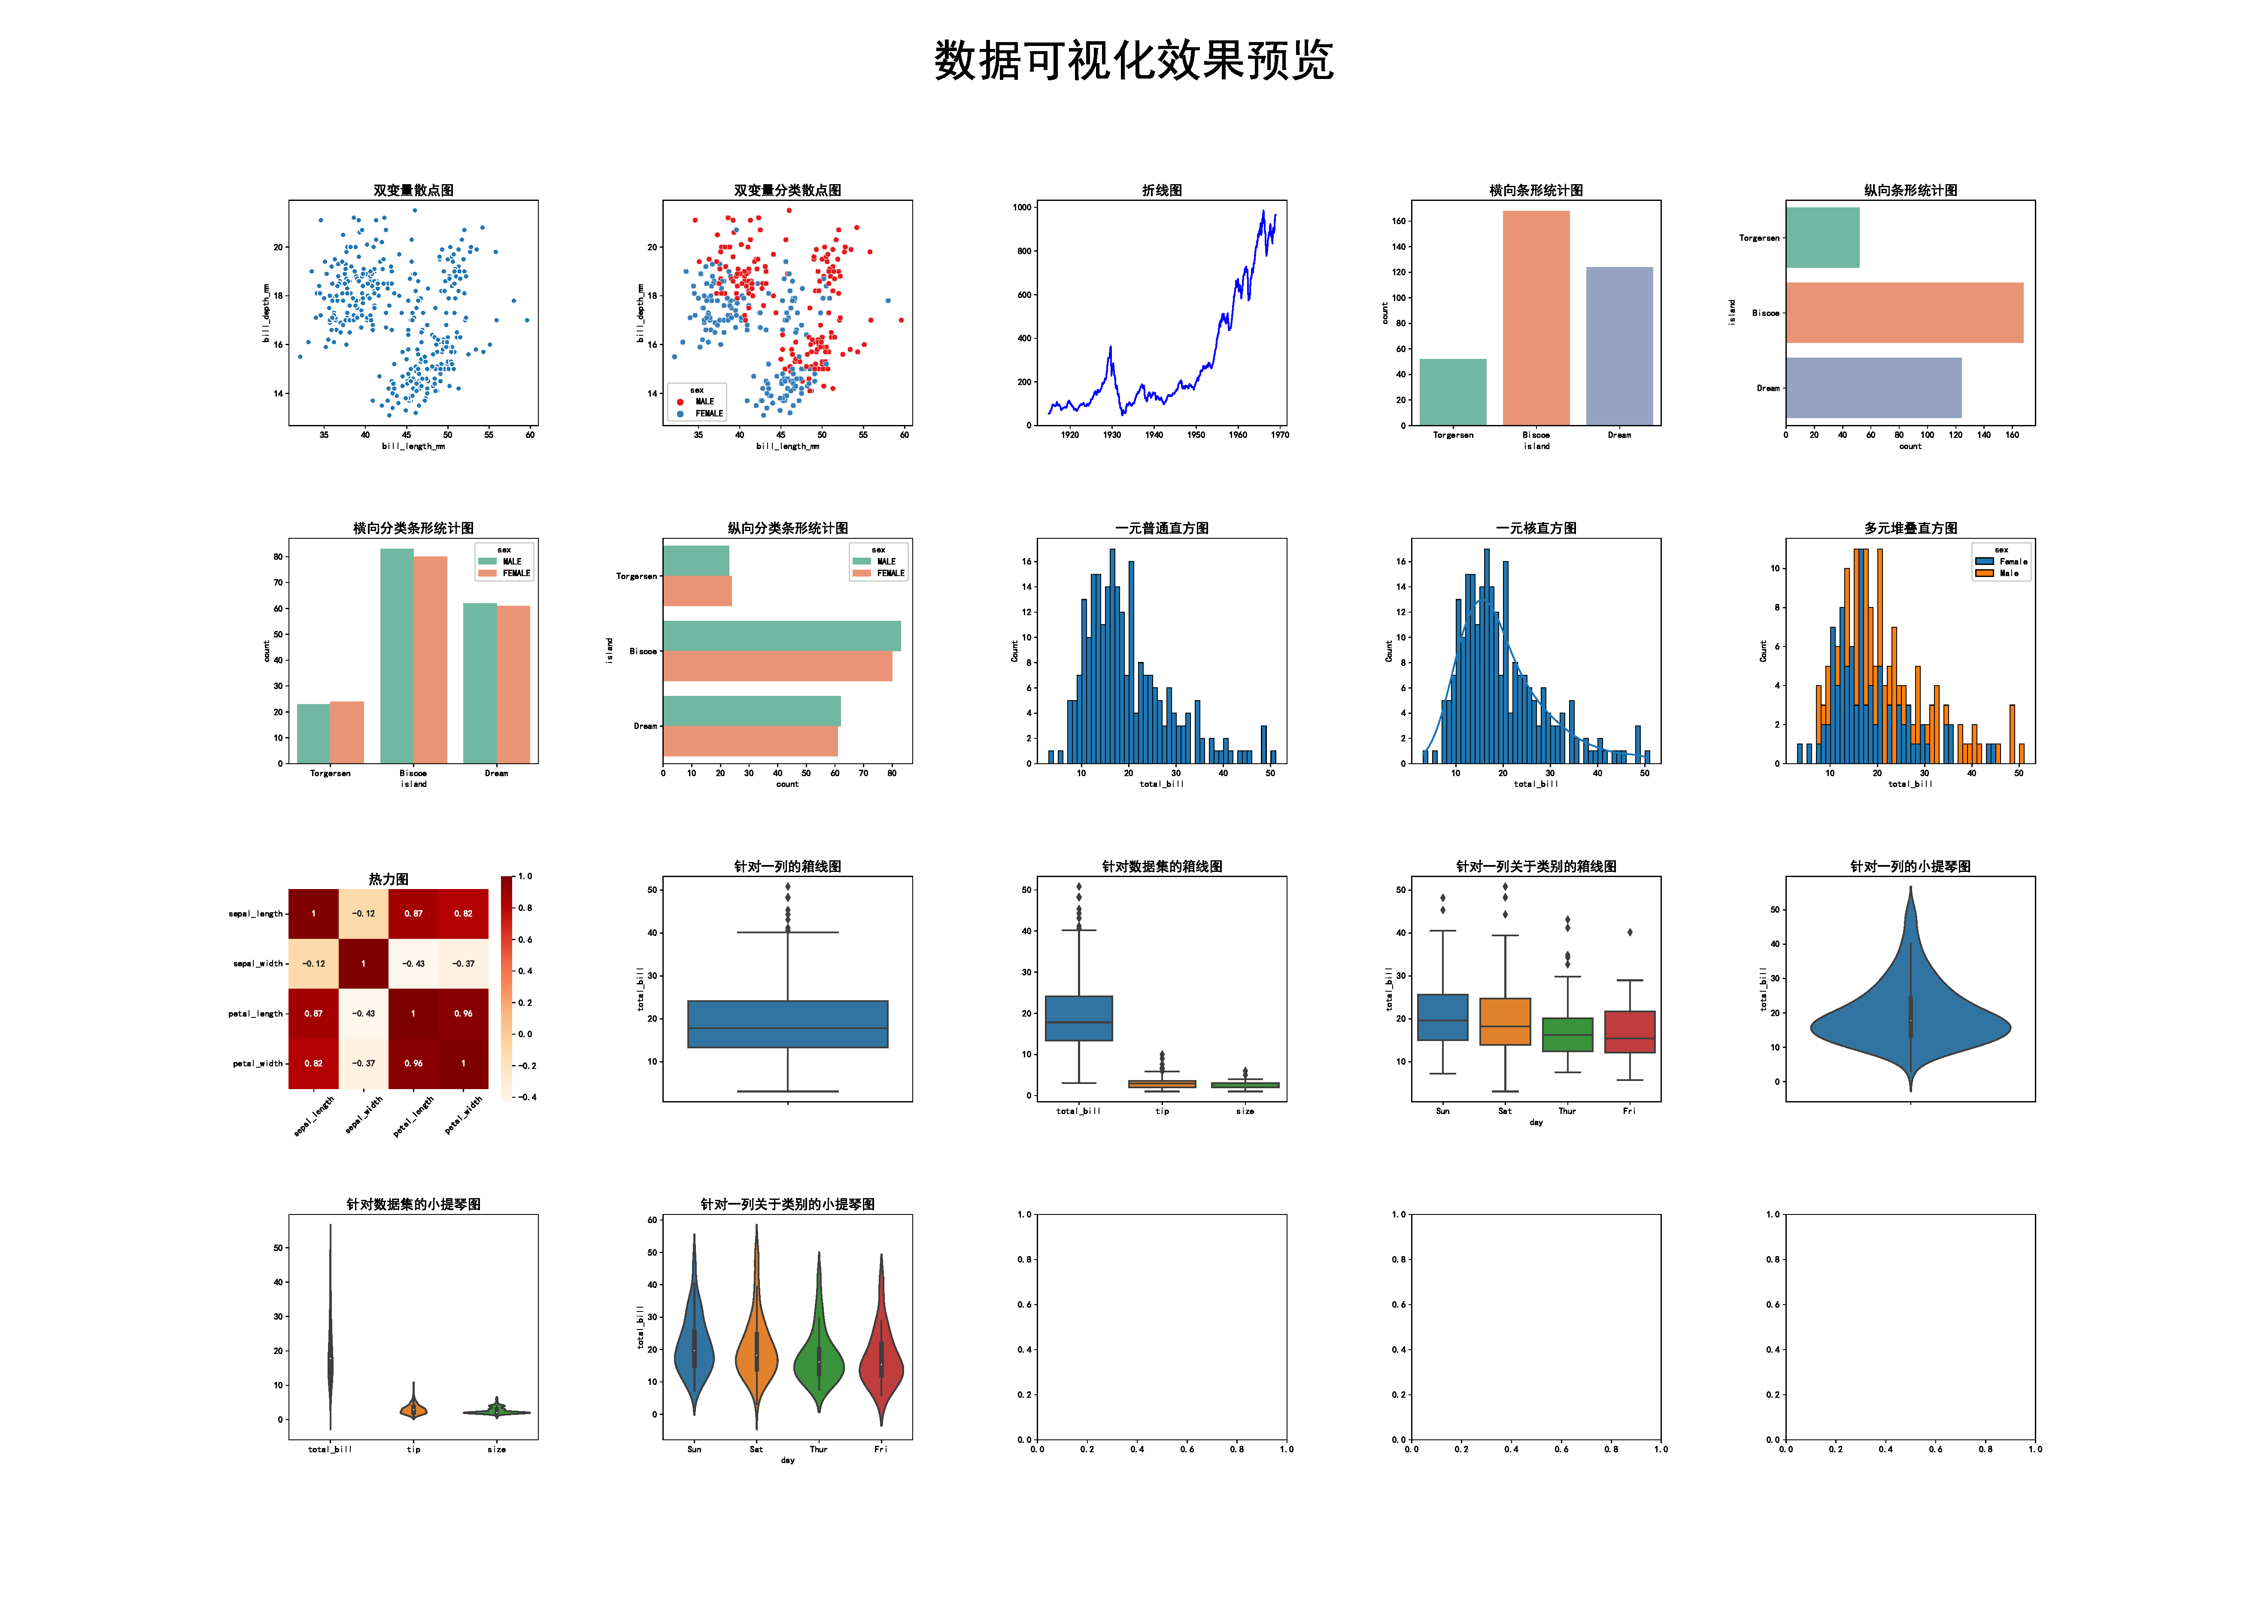
\includegraphics[width=1\textwidth]{1.eps}
	% 这是图注,也就是对图的解释,会在图片下方居中显示,请改成对应描述
	\caption{矢量图示例} 
	% 这是图片的标签,用于交叉引用该图片,务必全文唯一
	\label{fig2}
\end{figure}


矢量图也可以是pdf格式,比如本文的流程图——图~\ref{fig300}~就是pdf格式的。如果你希望在一行放多张图,可以参照图~\ref{fig100}~,~\ref{fig101}~:


\begin{figure}[H]
	\centering
	\begin{minipage}[t]{0.48\textwidth}
		\centering
		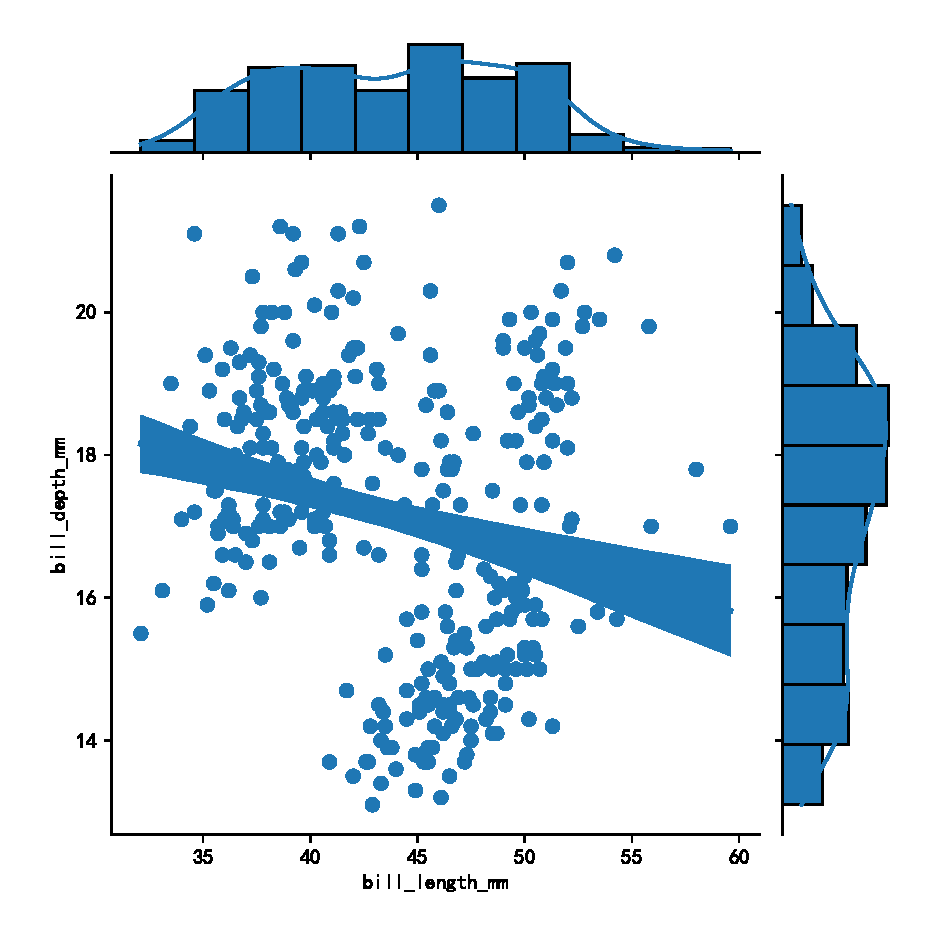
\includegraphics[width=1\textwidth]{test1.eps}
		\caption{左图}
		\label{fig100}
	\end{minipage}
	\begin{minipage}[t]{0.48\textwidth}
		\centering
		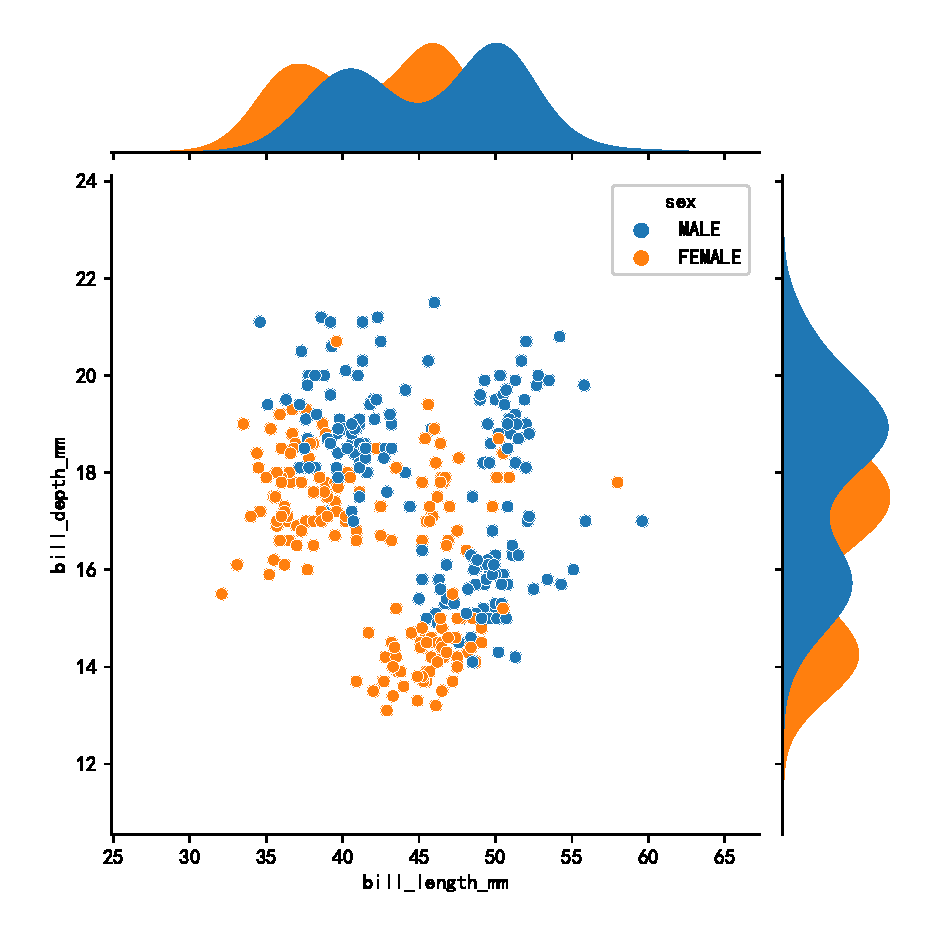
\includegraphics[width=1\textwidth]{test2.eps}
		\caption{右图}
		\label{fig101}
	\end{minipage}
\end{figure}

各位可以尝试一下,就会发现确有其事。

\subsection{插入表格}



论文中使用的表格一般是以三线表的形式呈现,三线表用处极多,必须掌握,而且在\LaTeX 中三线表是最麻烦的!我当初国赛通宵排版差点被三线表熬死,幸好孙竹清出手帮我搞定了,如表~\ref{table10}~:

\begin{table}[H]
	\centering
		\caption{这是表格标题。}
		\begin{tabular}{c c}  % 表有几列就要有几个c,c与c之间用空格隔开
			\toprule[1.5pt]   % 不要动
			% 表格内容,列与列之间用 & 隔开,一行内容写完了用 \\ 结束
			符号 & 含义  \\ 
			\midrule[1pt]     % 不要动
			$i=1,i=2$ & 分别表示高钾、铅钡玻璃 \\ 
			$j$ & 表示表中从二氧化硅($SiO_2$)到二氧化硫($SO_2$)中第$j$类化学物质 \\
			$z=1,z=2$ & 分别表示风化前和风化后 \\
			$x_1,x_2,x_3,x_4$ & 分别表示纹饰、类型、颜色、风化表面 \\
			$y_j$ & 表示第$j$类化学物质的含量 \\ 
			$\overline{y_j}$ & 表示第$j$类化学物质的平均含量 \\  
			\toprule[1.5pt]   % 不要动
		\end{tabular}
		\label{table10}
\end{table}

当然有时候也会遇到行合并单元格的情况,列合并的就比较少了,下面给出具体例子如表~\ref{table3}~:

\begin{table}[H]
	\centering
	\caption{对照组与实验组前、后测时间Mann-Whitney U检验}
	\begin{threeparttable}
		\begin{tabular}{c c c c c c c c c}
			\toprule[1.5pt]
			& 前测 & 平均值 & 标准差  & p值 & 后测 & 平均值 & 标准差  & p值 \\
			\midrule[1pt]
			
			
			\multirow{2}{*}{加法} & 对照组 & 某数据 & 某数据 & \multirow{2}{*}{某数据} & 对照组 & 某数据 & 某数据 & \multirow{2}{*}{某数据} \\
			
			& 实验组 & 某数据 & 某数据 &  & 实验组 & 某数据 & 某数据     \\
			
			\multirow{2}{*}{减法} & 对照组 & 某数据 & 某数据  & \multirow{2}{*}{某数据} & 对照组 & 某数据 & 某数据  & \multirow{2}{*}{某数据} \\
			
			& 实验组 & 某数据 & 某数据 &    & 实验组 & 某数据 & 某数据     \\
			\toprule[1.5pt]
		\end{tabular}
		\label{table3}
	\end{threeparttable}
\end{table}

我们在写论文时很可能会遇到极大量的计算结果需要放在三线表里,这个时候就很费心了,怎么办呢?在LaTeX中,你可以使用sidewaystable环境来创建一个横向表格,并且当表格横向放置不够时,自动将其旋转为竖向放置。你需要导入rotating宏包来使用这个环境。如表~\ref{table2}~所示:

\begin{table}[H]
	\centering
	\caption{这是一个横向的大表格}
	\begin{sideways}
		\begin{tabular}{c c c c c c c c c c c c c}
			\toprule[1.5pt]  
			列1 & 列2 & 列3 & 列1 & 列2 & 列3 列1 & 列2 & 列3 列1 & 列2 & 列3 列1 & 列2 & 列3 & 列1  \\
			\midrule[1pt]  
			内容1 & 内容2 & 内容3 & 内容1 & 内容2 & 内容3 & 内容1 & 内容2 & 内容3 &内容1 & 内容2 & 内容3 & 内容1  \\
			
			内容1 & 内容2 & 内容3 & 内容1 & 内容2 & 内容3 & 内容1 & 内容2 & 内容3 &内容1 & 内容2 & 内容3 & 内容1  \\
			
			内容1 & 内容2 & 内容3 & 内容1 & 内容2 & 内容3 & 内容1 & 内容2 & 内容3 &内容1 & 内容2 & 内容3 & 内容1 \\
			
			内容1 & 内容2 & 内容3 & 内容1 & 内容2 & 内容3 & 内容1 & 内容2 & 内容3 &内容1 & 内容2 & 内容3 & 内容1 \\
			
			内容1 & 内容2 & 内容3 & 内容1 & 内容2 & 内容3 & 内容1 & 内容2 & 内容3 &内容1 & 内容2 & 内容3 & 内容1  \\
			
			内容1 & 内容2 & 内容3 & 内容1 & 内容2 & 内容3 & 内容1 & 内容2 & 内容3 &内容1 & 内容2 & 内容3 & 内容1  \\
			
			内容1 & 内容2 & 内容3 & 内容1 & 内容2 & 内容3 & 内容1 & 内容2 & 内容3 &内容1 & 内容2 & 内容3 & 内容1  \\
			
			内容1 & 内容2 & 内容3 & 内容1 & 内容2 & 内容3 & 内容1 & 内容2 & 内容3 &内容1 & 内容2 & 内容3 & 内容1  \\
			
			内容1 & 内容2 & 内容3 & 内容1 & 内容2 & 内容3 & 内容1 & 内容2 & 内容3 &内容1 & 内容2 & 内容3 & 内容1  \\
			
			内容1 & 内容2 & 内容3 & 内容1 & 内容2 & 内容3 & 内容1 & 内容2 & 内容3 &内容1 & 内容2 & 内容3 & 内容1  \\
			
			内容1 & 内容2 & 内容3 & 内容1 & 内容2 & 内容3 & 内容1 & 内容2 & 内容3 &内容1 & 内容2 & 内容3 & 内容1  \\
			\toprule[1.5pt] 
			% 继续添加更多行和列
		\end{tabular}
	\end{sideways}
	\label{table2}
\end{table}
